\documentclass[a4paper]{article}




\usepackage[margin=1in]{geometry} % full-width

% AMS Packages
\usepackage{amsmath}
\usepackage{amsthm}
\usepackage{amssymb}

% Unicode
\usepackage[utf8]{inputenc}
\usepackage{hyperref}
\hypersetup{
	unicode,
%	colorlinks,
%	breaklinks,
%	urlcolor=cyan, 
%	linkcolor=blue, 
	pdfauthor={Author One, Author Two, Author Three},
	pdftitle={A simple article template},
	pdfsubject={A simple article template},
	pdfkeywords={article, template, simple},
	pdfproducer={LaTeX},
	pdfcreator={pdflatex}
}

% Vietnamese
%\usepackage{vntex}

% Natbib
\usepackage[sort&compress,numbers,square]{natbib}
\bibliographystyle{mplainnat}

% Theorem, Lemma, etc
\theoremstyle{plain}
\newtheorem{theorem}{Theorem}
\newtheorem{corollary}[theorem]{Corollary}
\newtheorem{lemma}[theorem]{Lemma}
\newtheorem{claim}{Claim}[theorem]
\newtheorem{axiom}[theorem]{Axiom}
\newtheorem{conjecture}[theorem]{Conjecture}
\newtheorem{fact}[theorem]{Fact}
\newtheorem{hypothesis}[theorem]{Hypothesis}
\newtheorem{assumption}[theorem]{Assumption}
\newtheorem{proposition}[theorem]{Proposition}
\newtheorem{criterion}[theorem]{Criterion}
\theoremstyle{definition}
\newtheorem{definition}[theorem]{Definition}
\newtheorem{example}[theorem]{Example}
\newtheorem{remark}[theorem]{Remark}
\newtheorem{problem}[theorem]{Problem}
\newtheorem{principle}[theorem]{Principle}

\usepackage{graphicx, color}
\graphicspath{{fig/}}

%\usepackage[linesnumbered,ruled,vlined,commentsnumbered]{algorithm2e} % use algorithm2e for typesetting algorithms
\usepackage{algorithm, algpseudocode} % use algorithm and algorithmicx for typesetting algorithms
\usepackage{mathrsfs} % for \mathscr command



% Author info

\begin{document}
    \begin{titlepage}
        \centering
        {
\includegraphics[width=0.2\textwidth]{logo}\par}
        \vspace{1cm}
        {\bfseries\LARGE Universidad Castilla La Mancha \par}
        \vspace{1cm}
        {\scshape\Large Ingeniería informática \par}
        \vspace{3cm}
        {\scshape\Huge linear data structure \par}
        \vspace{3cm}
        {\itshape\Large Data Structure laboratory\par}
        \vfill
        {\Large Authors: \par}
        {\Large Andrés González Varela  \par Juan Gigante Rios\par  María Jesús Dueñas Recuero }
        \vfill
        {\Large October 2021 \par}
    \end{titlepage}
	

\newpage
	\tableofcontents
	\newpage
	\section{Stack}
        \subsection{Problem description}
        There is a data file containing natural numbers. This file will be read number by number and you must apply the following treatment:
        \begin{itemize}
            \item Place the first number on a first stack.
            \item The following numbers will be compared with the one on top of the first stack. When the addition of the read number with the number on top is nine, you must insert two times the lower of the two on a second stack and remove the number on top of the first stack.
            \item If the addition is not nine, the read number must be placed on the first stack. Once finished the first treatment, you must empty the second stack number by number in a way that, when two or more consecutive numbers add up to nine or more, a nine must be placed on a third stack.
        \end{itemize}
        The final output of the program will be the number of nines contained in the third stack.

     \subsection{Approach}
        The main idea to develop this project is to divide it into classes according to each of the functions. That is why, we have created a \textbf{ReadFile} class which is in charge of reading the file provided to us for the practice, the \textbf{Problem} class where most of the code will be developed solving the problem and finally, the \textbf{Main} class where only calls to methods of the classes will be made and the result will be shown by console. All this by means of an object oriented programming.


        \subsubsection{Developing ReadFile class}
        \begin{itemize}
            \item \textbf{read-File}\par
            In order to read the file given to us, and taking into account that the practices consist in the use and handling of stacks, we have considered storing the information of this file in a stack,\textbf{aux-number-Stack-file }.

             As when storing it in a stack the information will be stored inversely to how we read it, we use another stack ,\textbf{number-Stack-File}, to re-invert the information and make it look as it is read in the file so that it is easier to work with.Therefore, this method will return a stack with the information from the file figure[1].\newline
             \item \textbf{Read-file constructor}\par
           The constructor method is a special method to create and initialise an object created from a class, in our case to create an object of the class "ReadFile".
        \end{itemize}
        
             \begin{figure}[h]
                \centering
                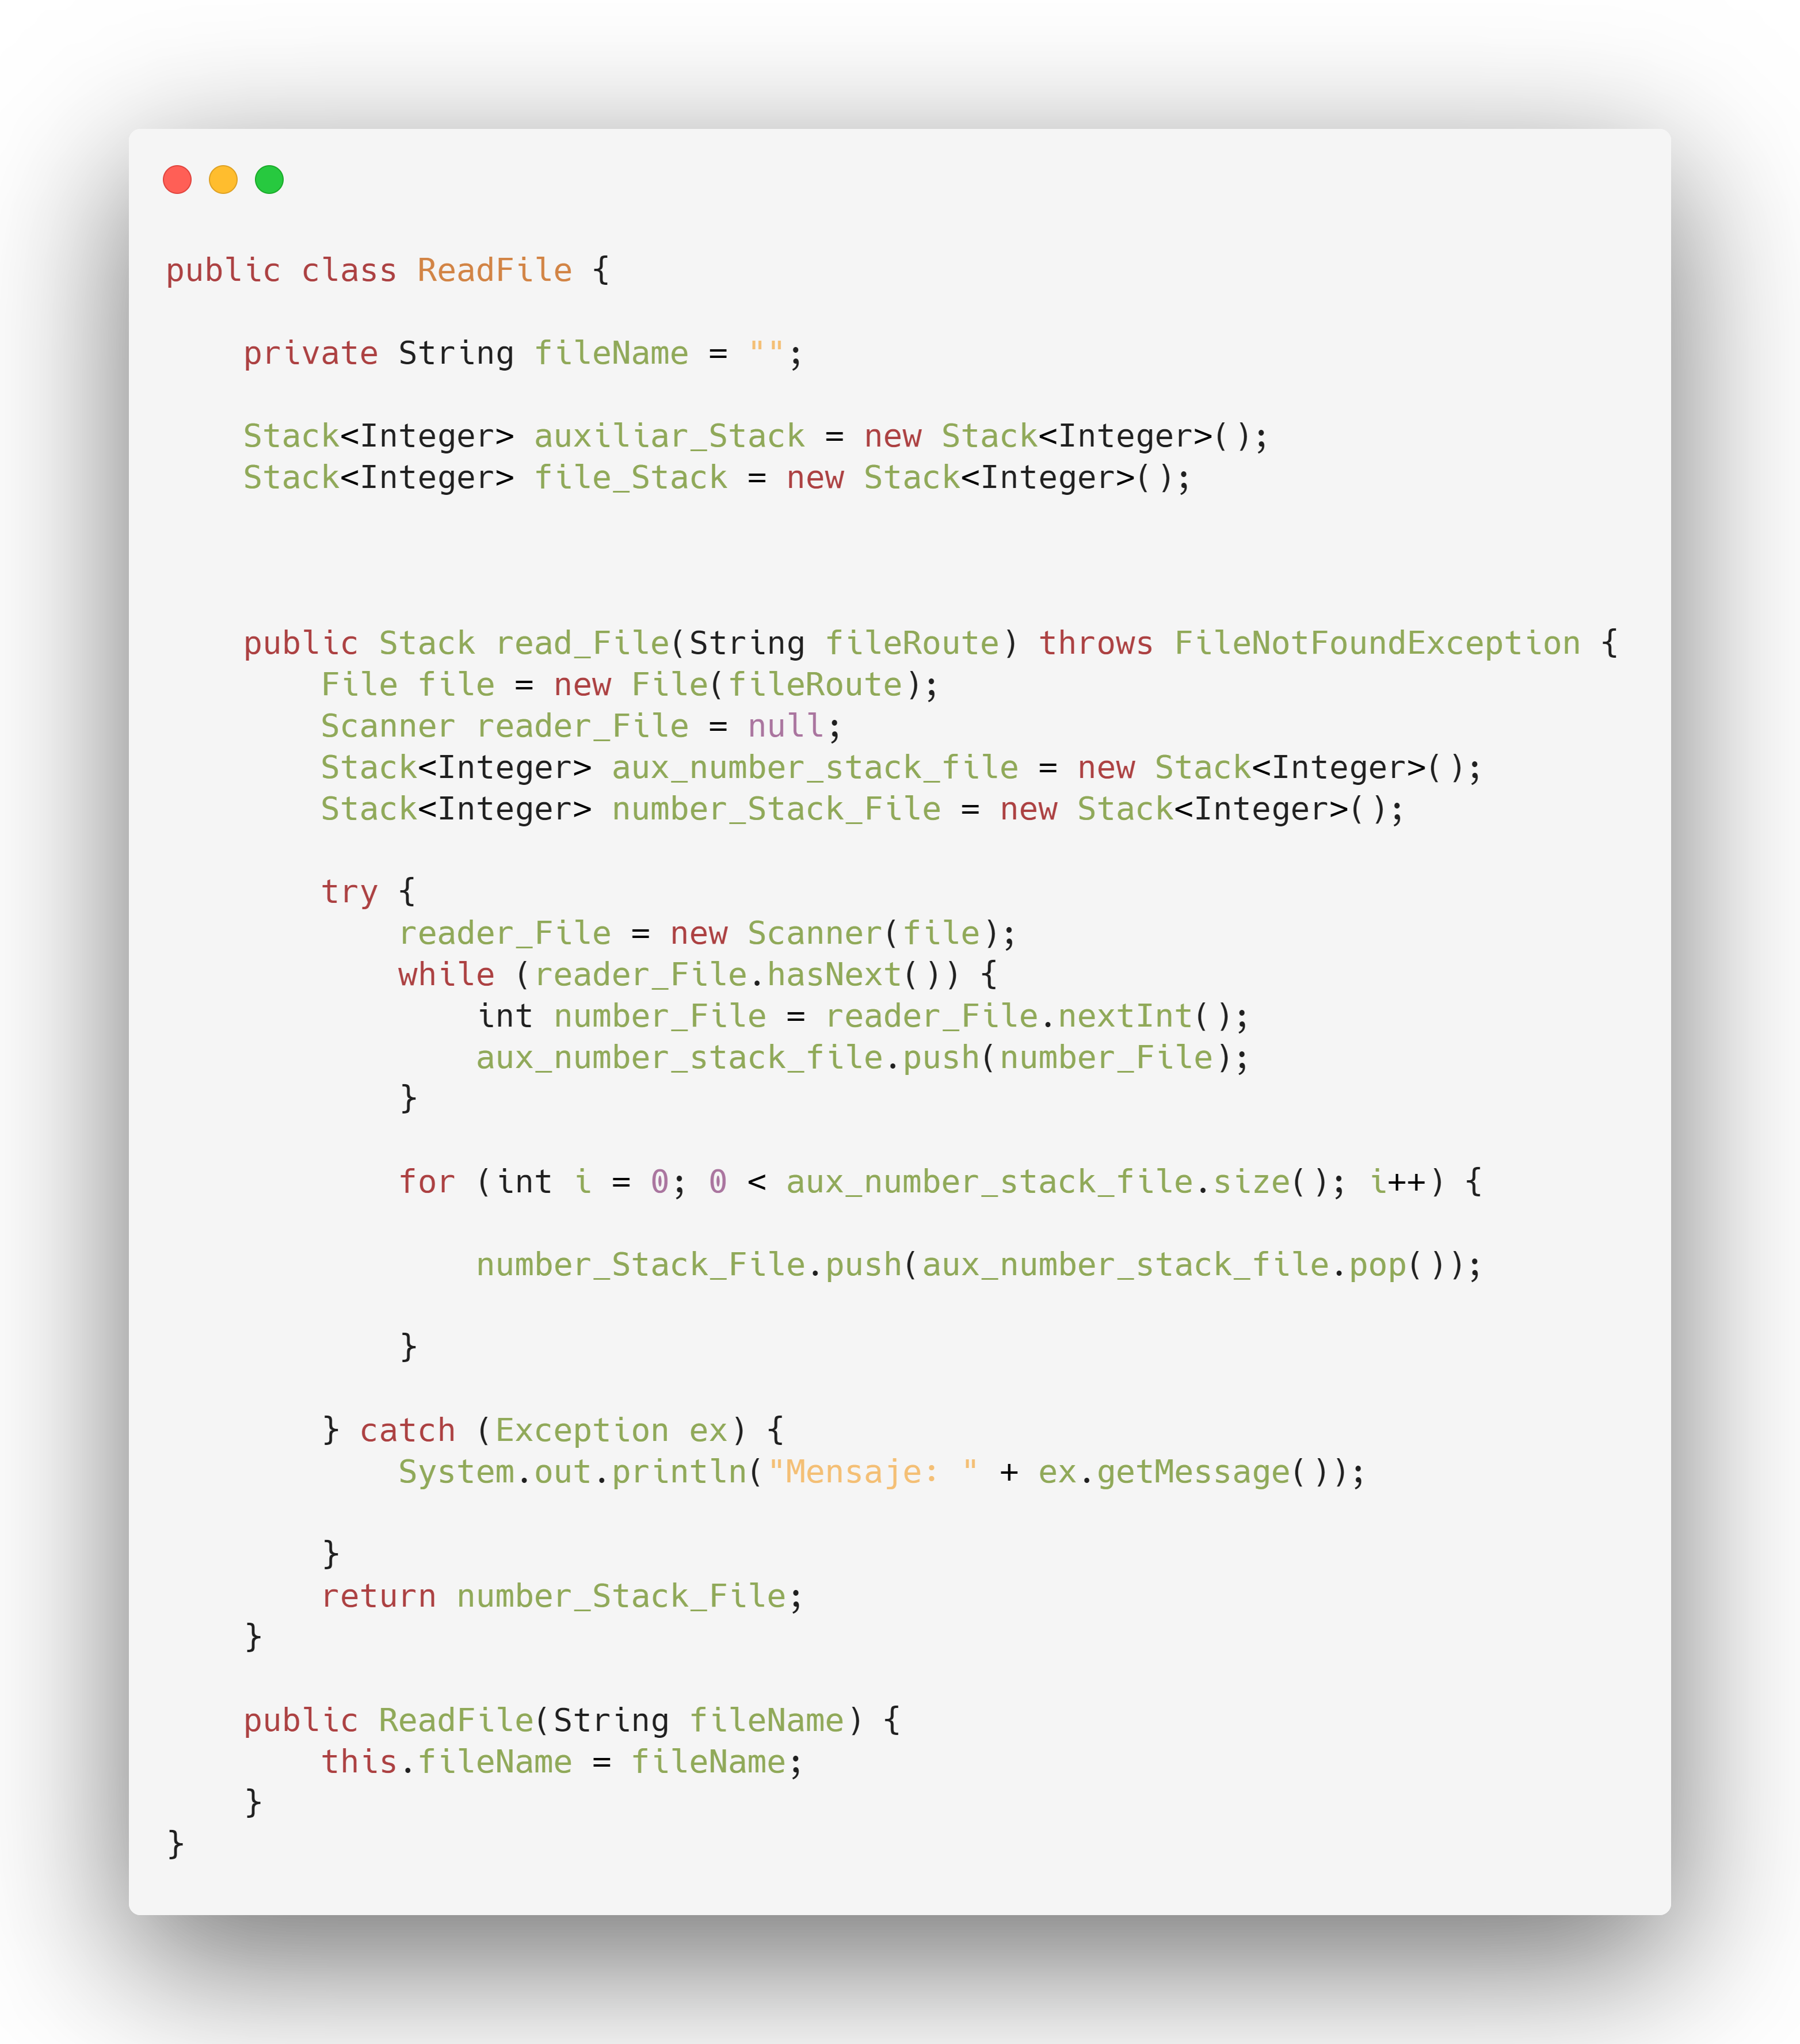
\includegraphics[width=300pt\textwidth]{read-file.png}
                \caption{Code of the ReadFile class}
                \label{fig:mesh1}
            \end{figure}
        

\newpage
        \subsubsection{Developing Problem class}
            \begin{itemize}
                \item \textbf{fill-Stacks}
                This method is the body of the class, it is where we try to solve the practice. The main idea of this method is to read the file-stack (containing the numbers to be read) where the first number of this file is put into the first-stack and the last top number in this row is added to the file-stack.\par

                Afterwards, if the sum is nine, the smallest sum will be added to the second-stack, otherwise it will return to the first-stack.\par

                We use the FileNotFoundException and EmptyStackException exceptions to control that the file is found and that if the stack is empty it does not crash the program, respectively.\par

                As an important clarification we have used the condition if(i==0) in line 28, to control that only one file-stack number is inserted in each iteration since it was giving us problems if we didn't control it.\par
                \begin{figure}[h]
                     \centering
                     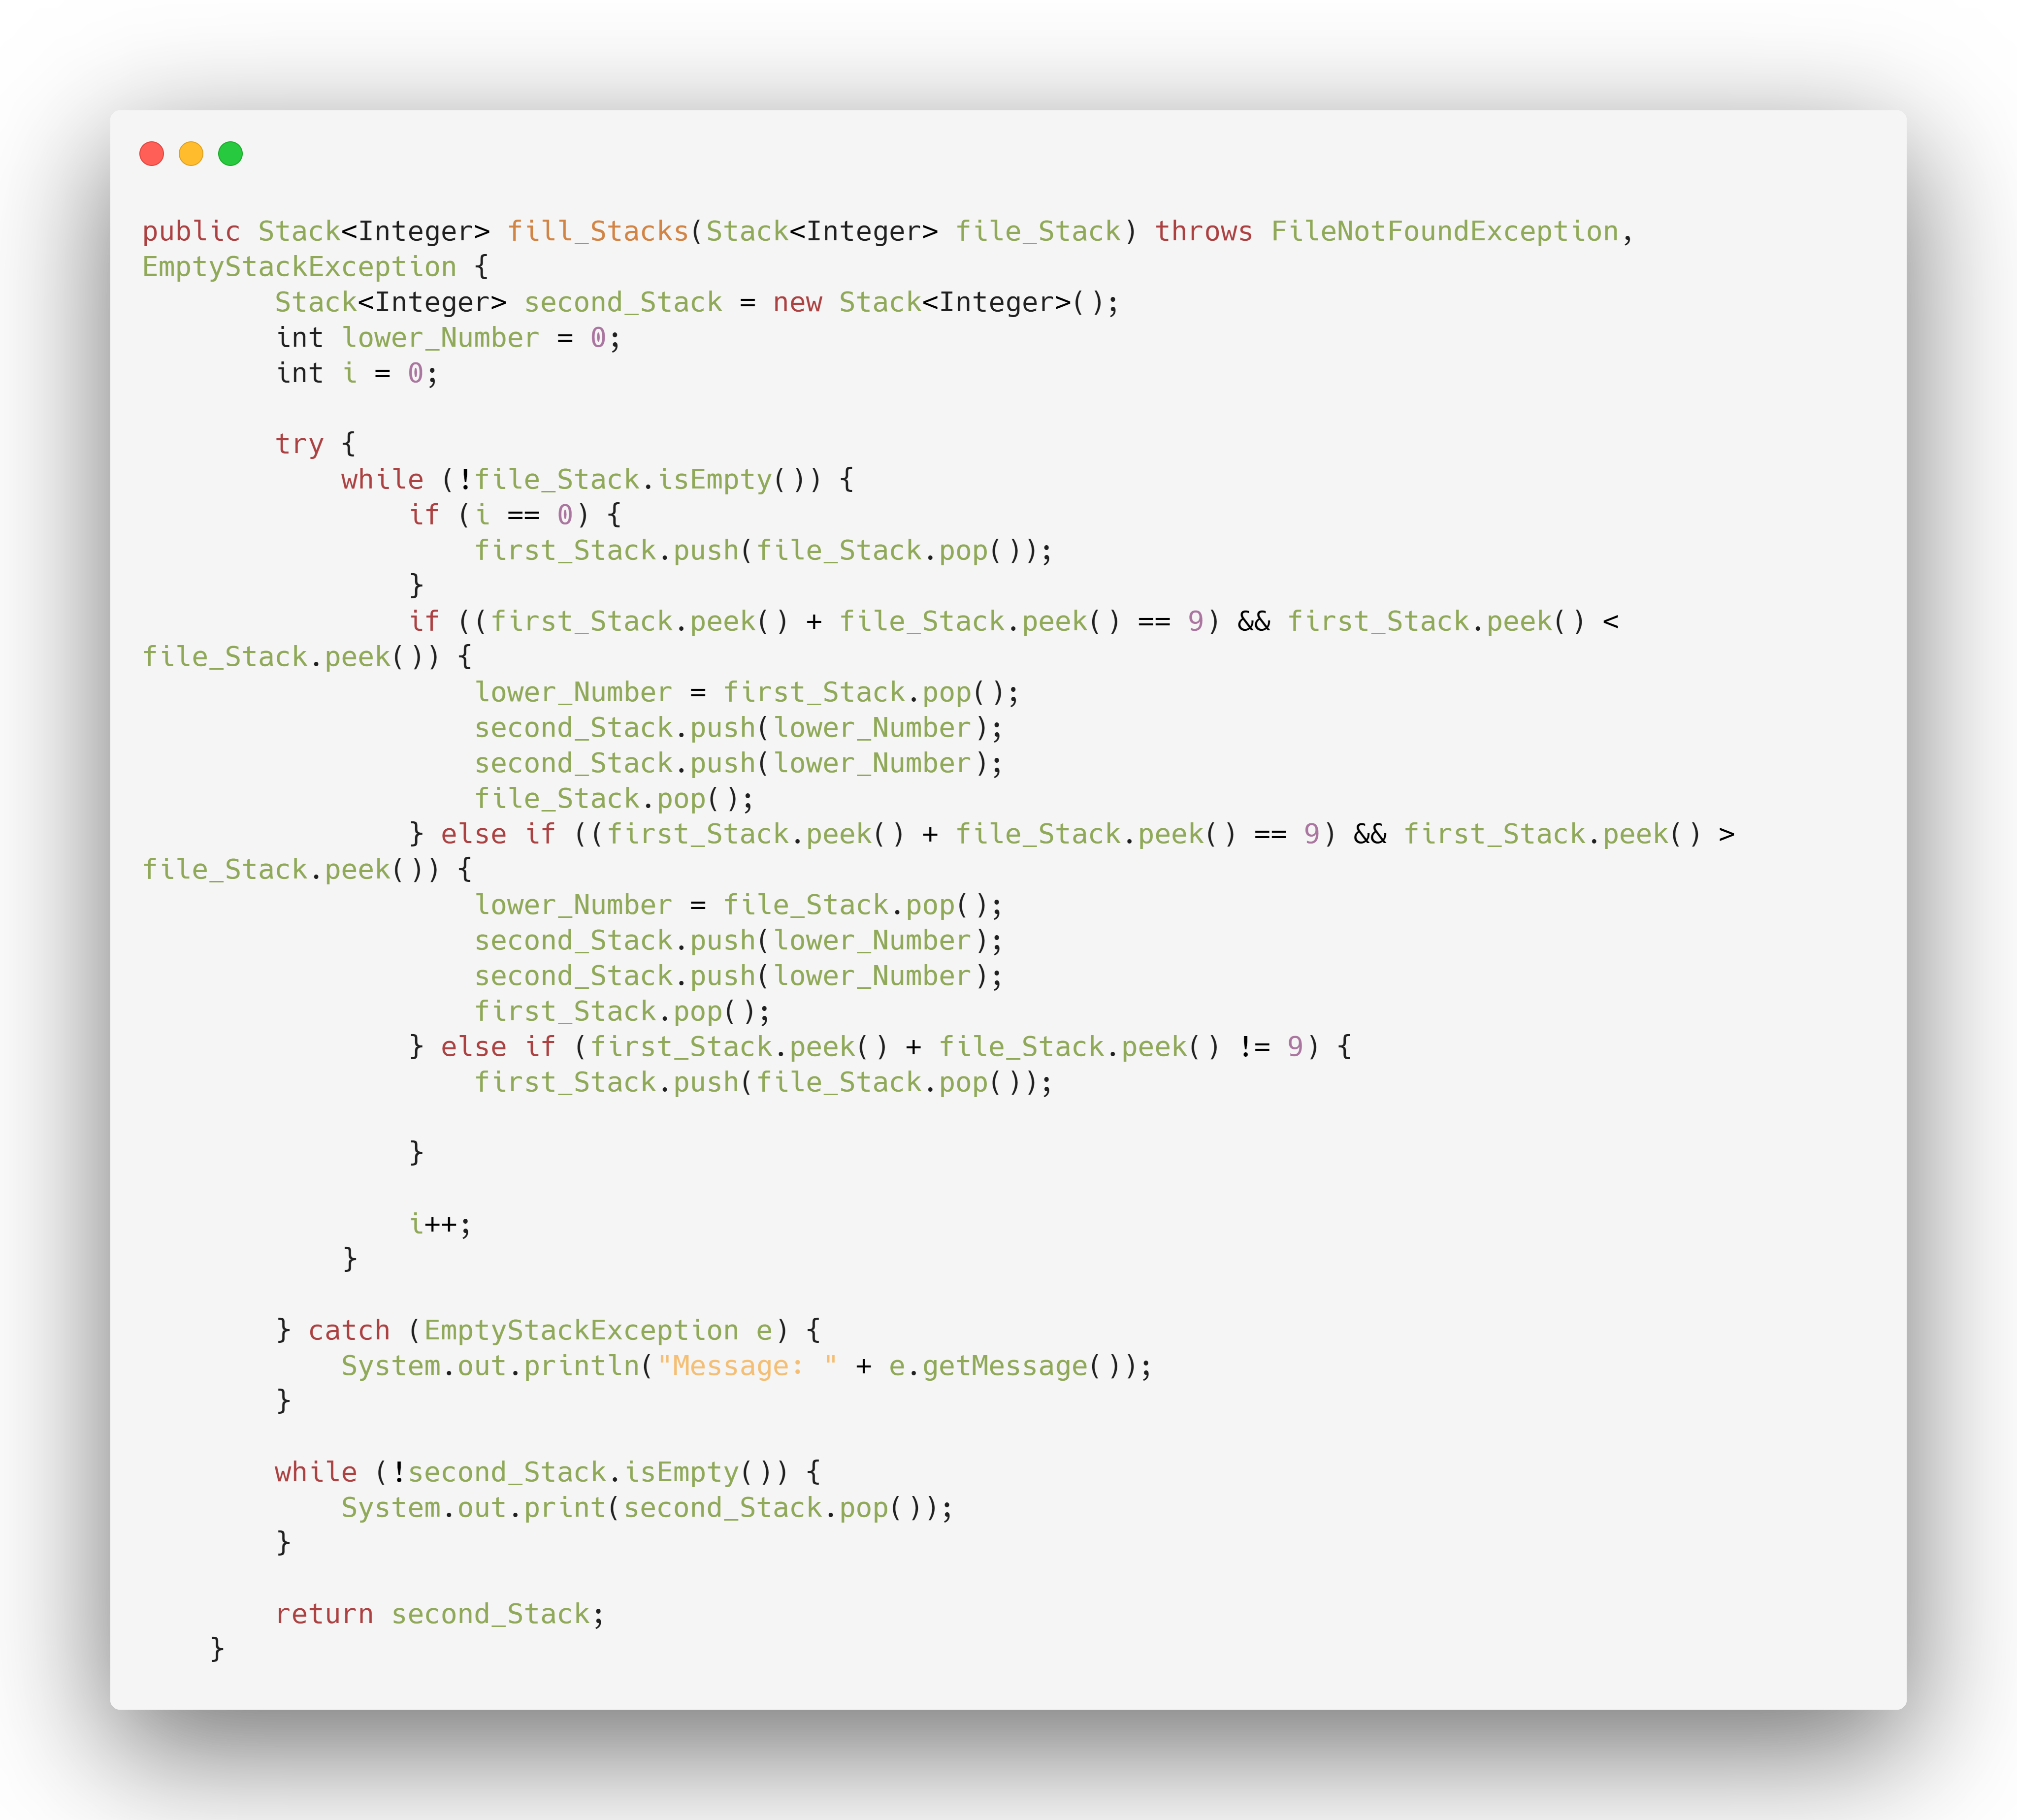
\includegraphics[width=300pt\textwidth]{fill-stack.png}
                     \caption{Code of the fill-stack method}
                     \label{fig:mesh1}
                \end{figure}

\newpage
                \item \textbf{counter-nine}
                This is the second part of the program where the sum of all the numbers in the second-stack is carried out. If the sum between two or more addends is nine or more, a nine is added to the third-stack.[Figure 3]
                \begin{figure}[h]
                     \centering
                     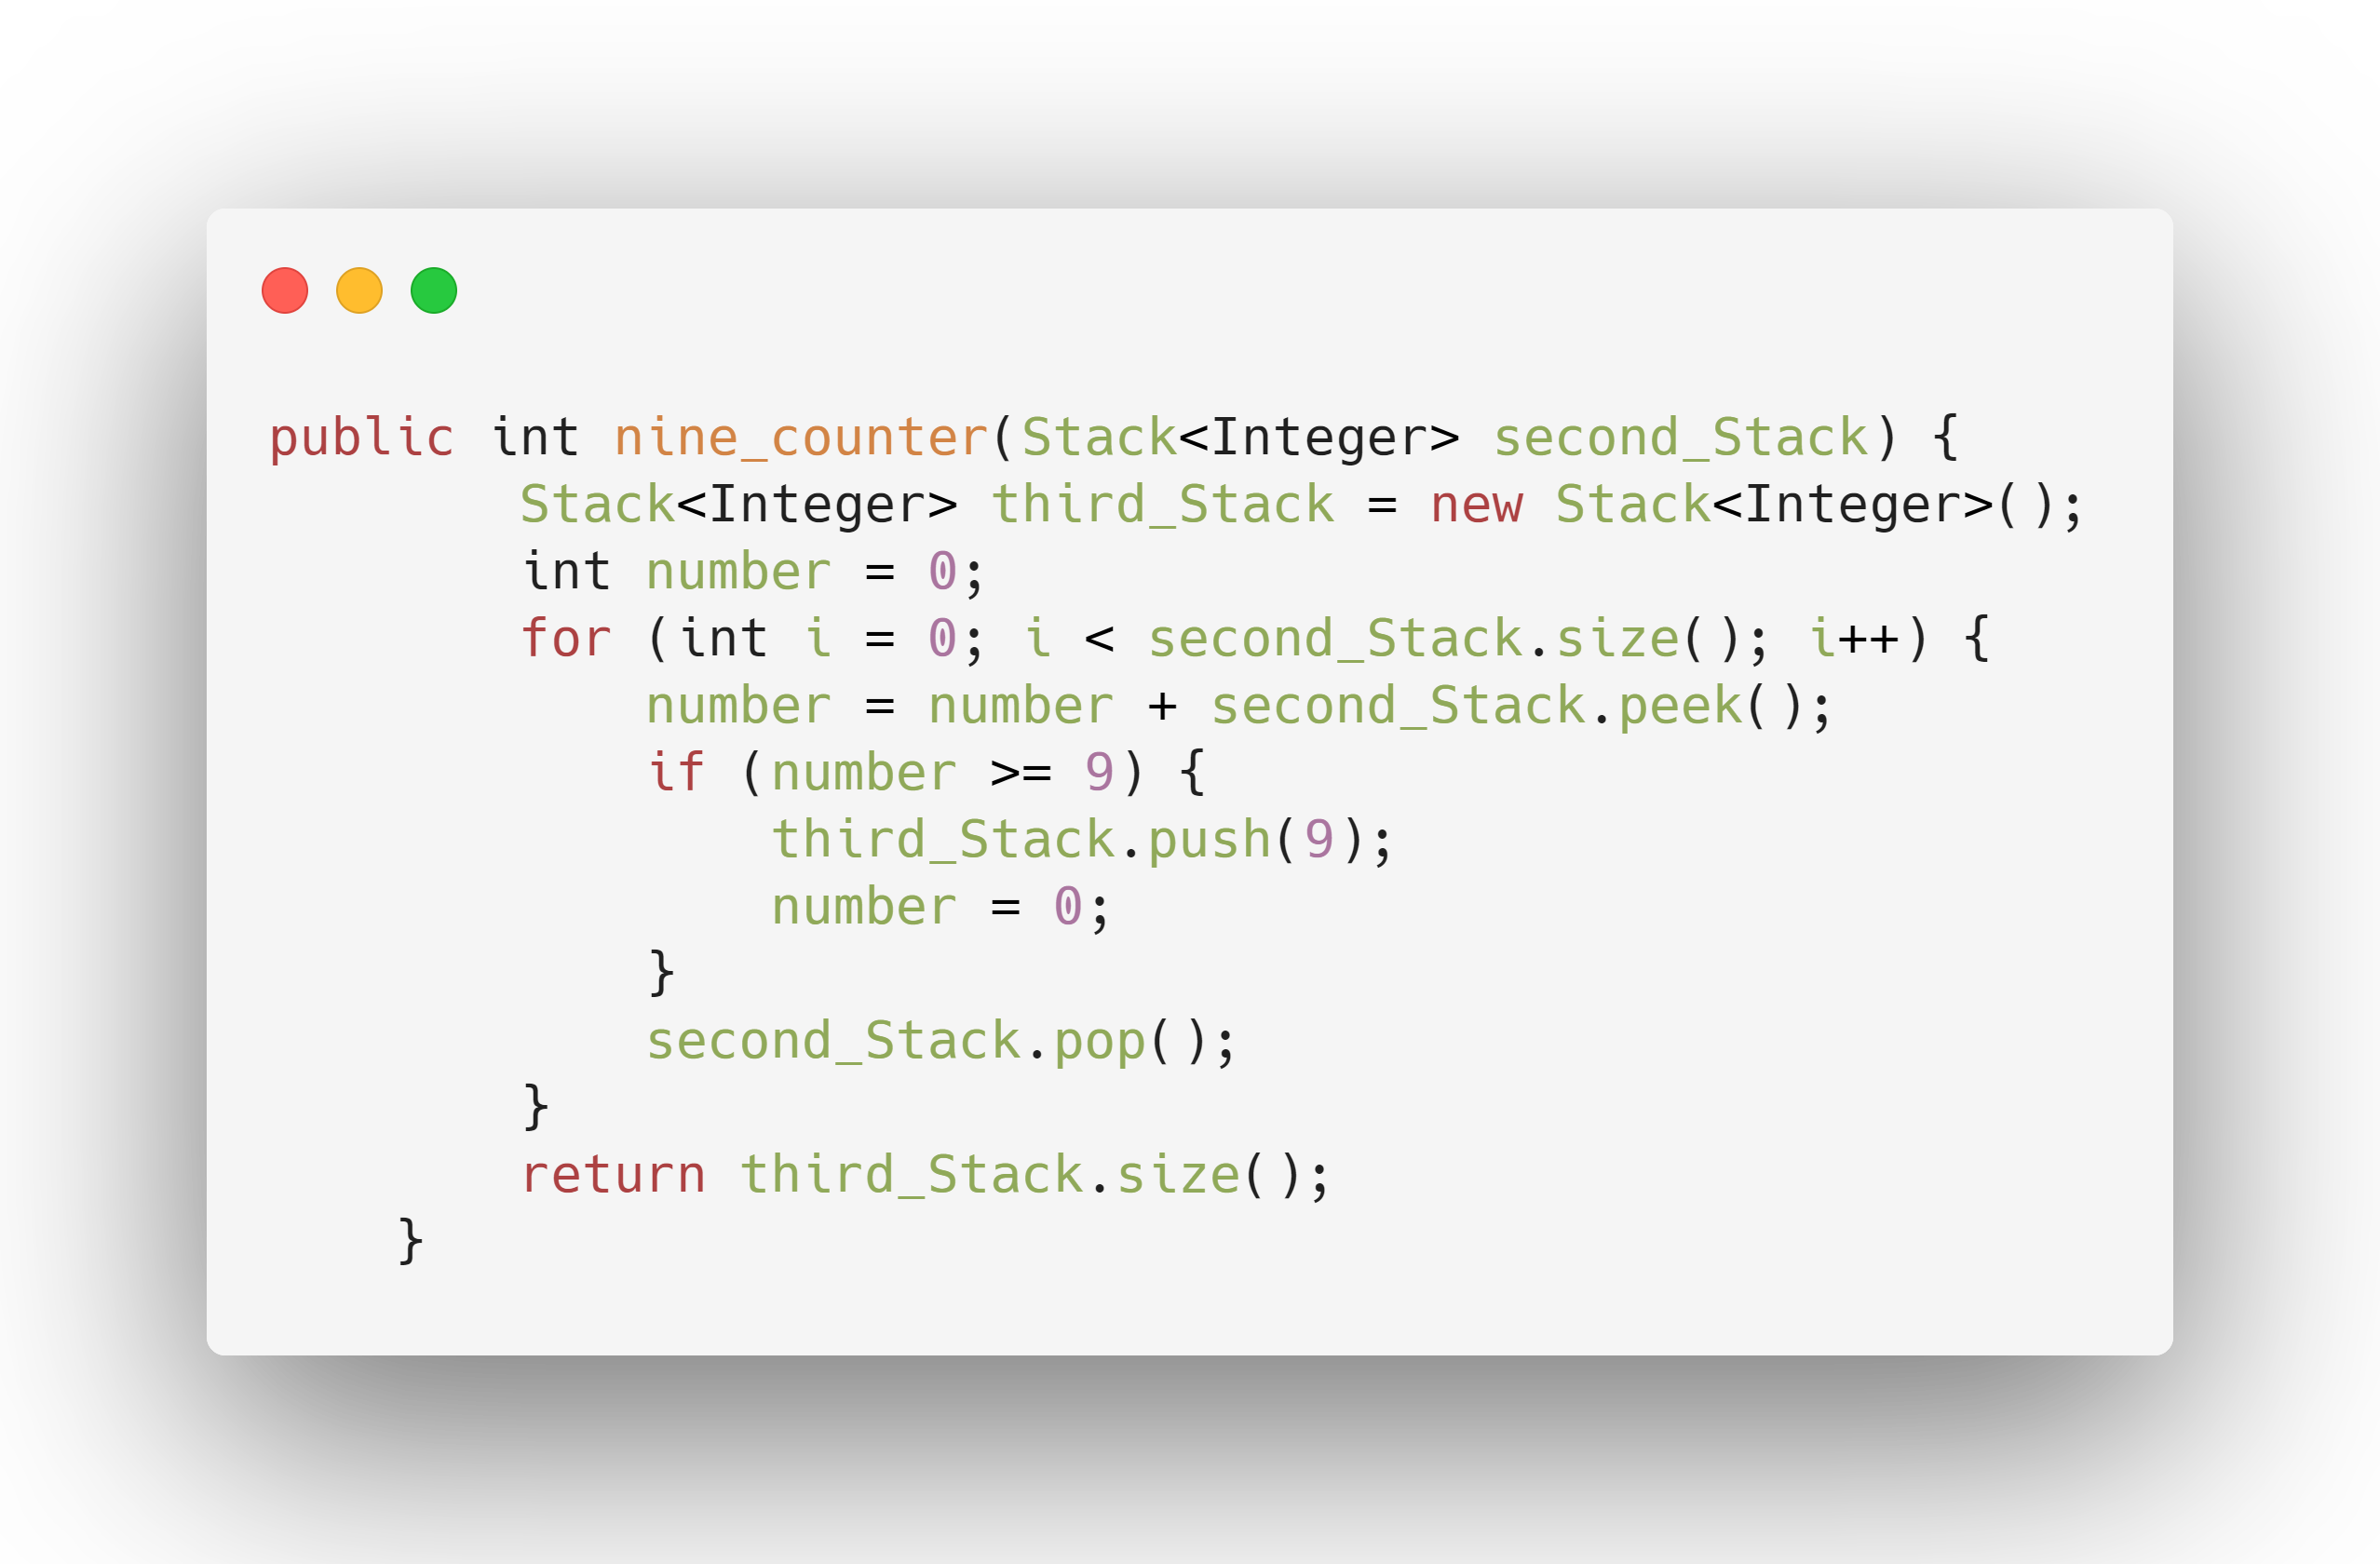
\includegraphics[width=300pt\textwidth]{counter-nine.png}
                     \caption{Code of the nine-counter method}
                     \label{fig:mesh1}
                \end{figure}

                \item \textbf{Problem [constructor]}
                The constructor method is a special method to create and initialise an object created from a class, in our case to create an object of the class "Problem".

            \end{itemize}
        \subsubsection{EmptyStackException}
        This is the custom exception class that we have created. This exception will be thrown when any stack is empty and will prevent the program from crashing.
        \subsubsection{Developing Main class}
        In the main class we have created 3 stacks that, which we will use in the whole problem, then after this we also create and object from the class problem for work with it latelly We ask for the direction of the file in your computer (C://naturales.dat.txt) for example, and the Scanner gets the direction of the file.\par When we obtain the direction of it we create a readFile object and with this we invoke the method read form the class readFile and we will obtain the stack with all the numbers. \par
    After this we fill the second stack with the method fill-Stacks from the class Problem.Last of all we take the method nine-counter to count the amount of 9's that we have in the third stack
        \begin{figure}[h]
            \centering
            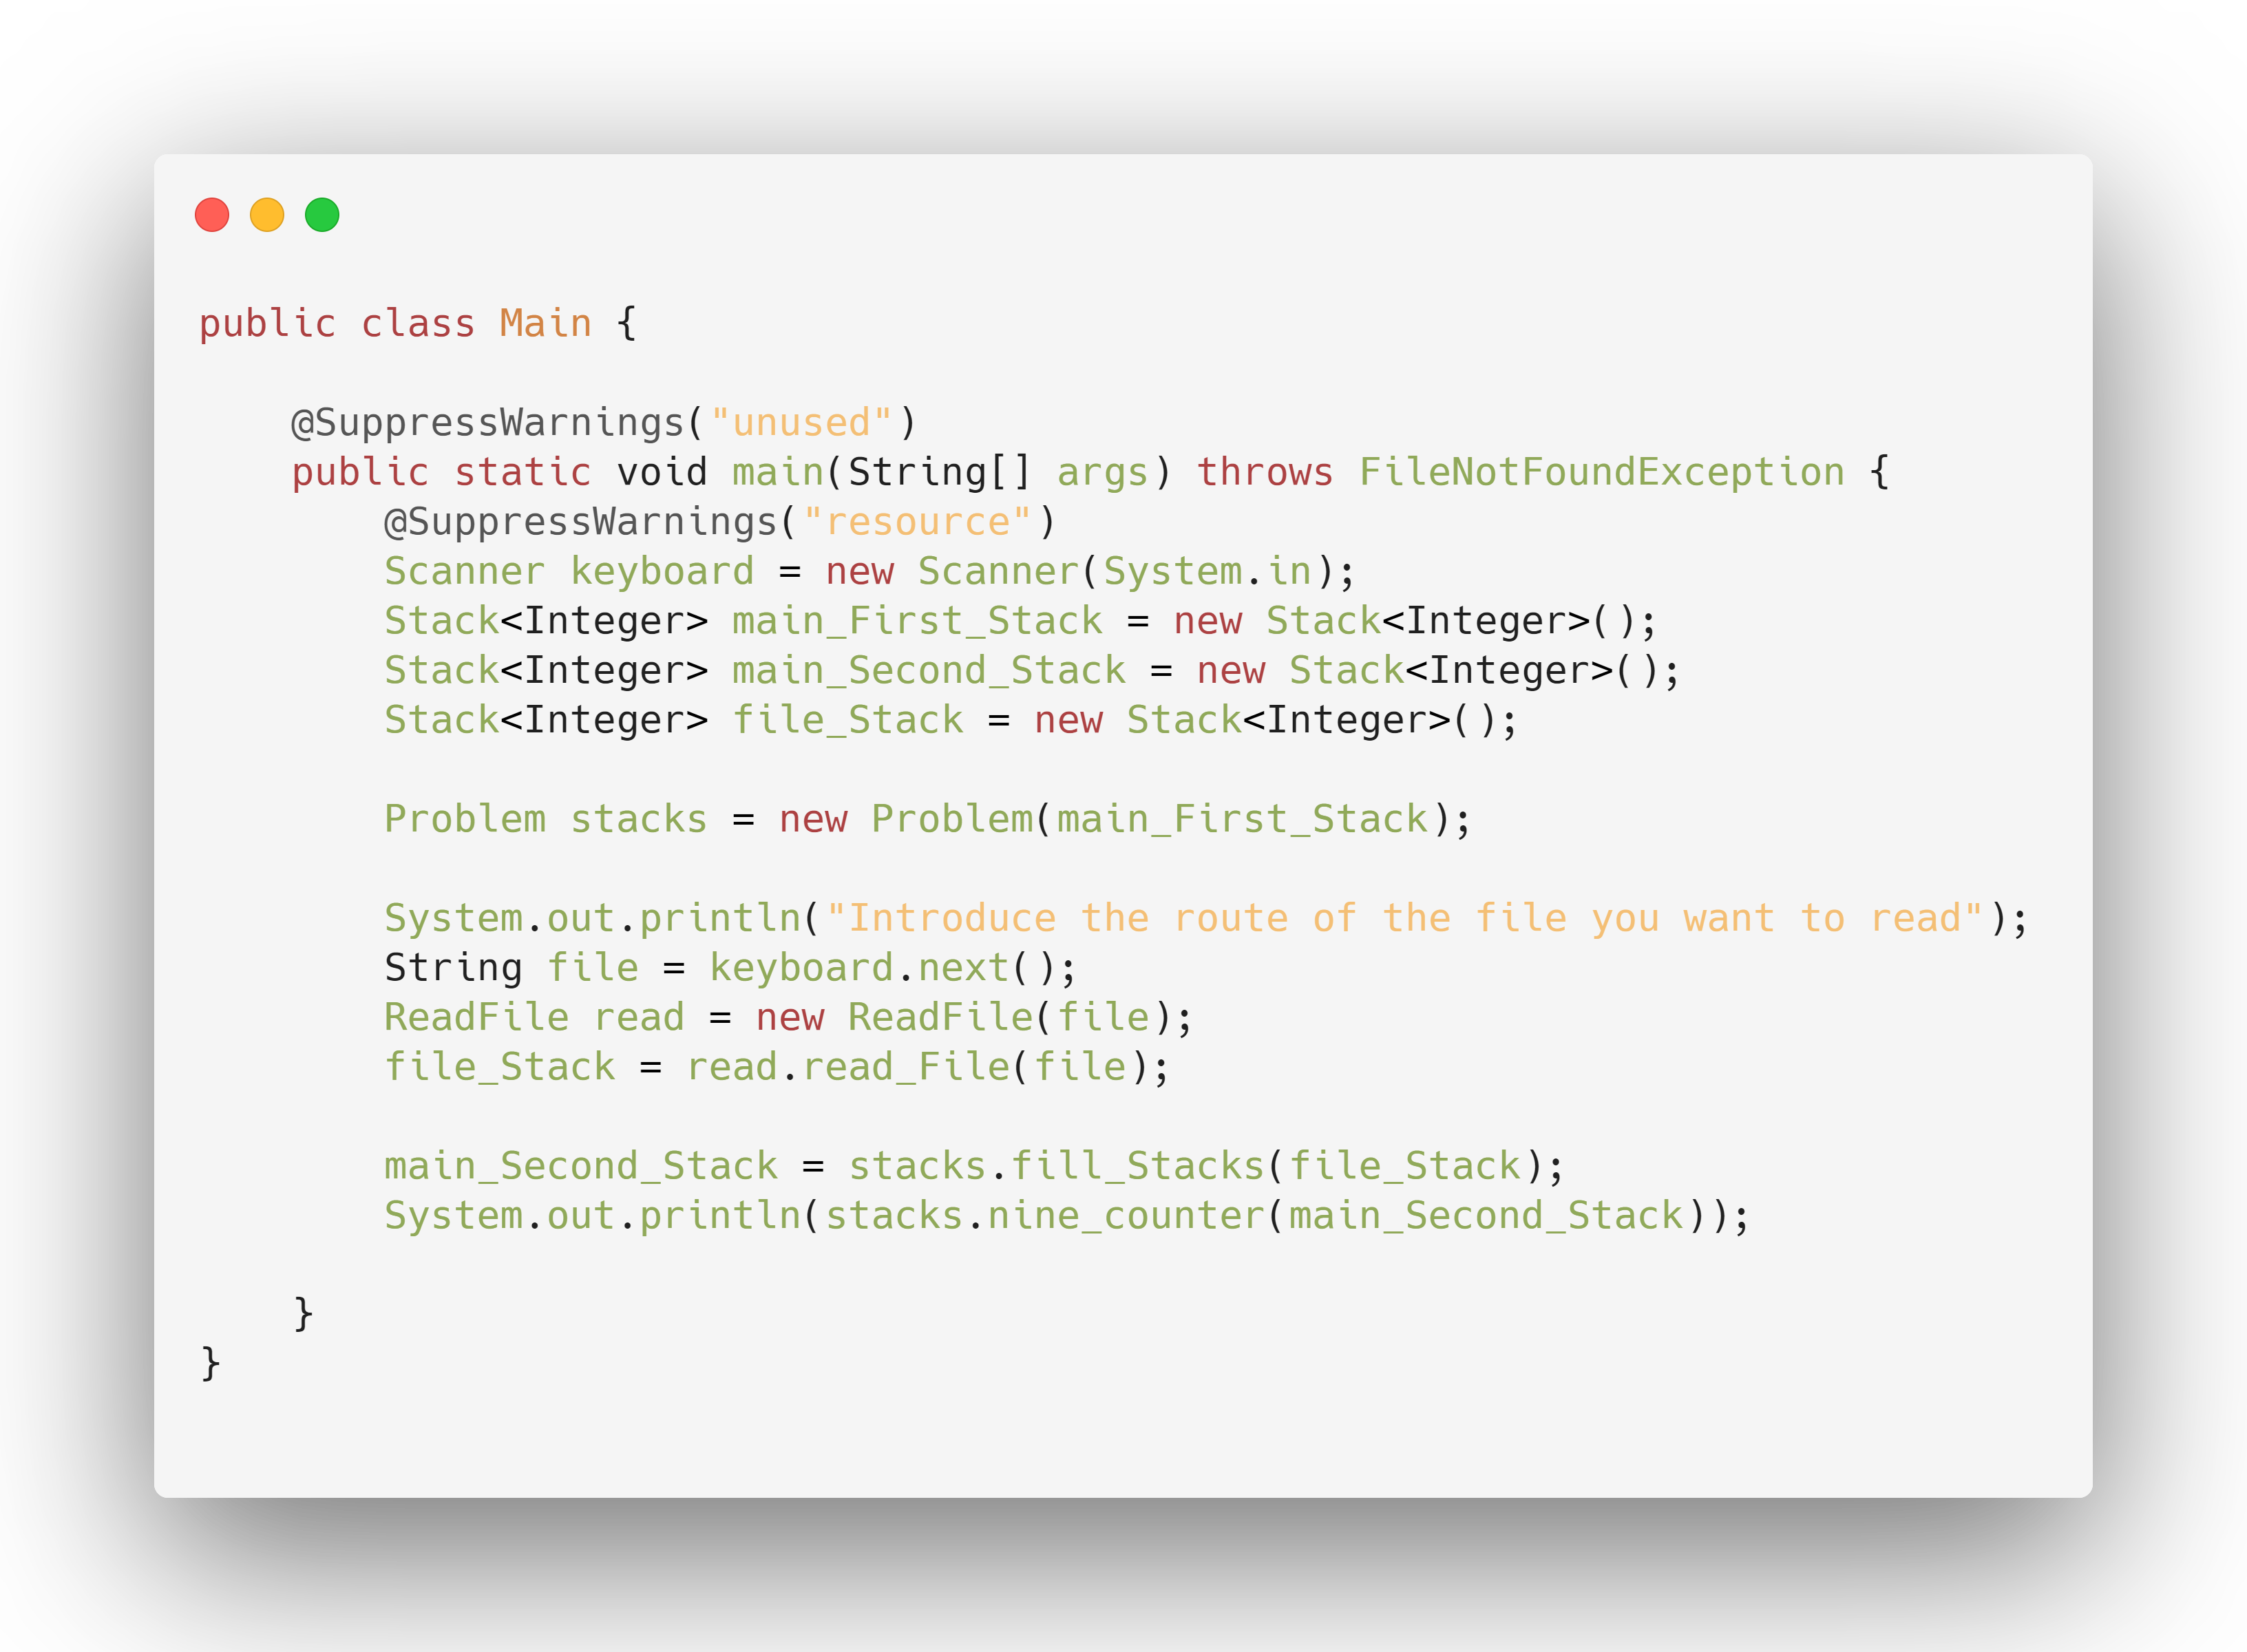
\includegraphics[width=300pt\textwidth]{main-stacks.png}
            \caption{Code of the Main class}
             \label{fig:mesh1}
        \end{figure}
        
        
   \subsection{Tecnical requirement and running}
        \subsubsection{Generation bat}
        In order to be able to run the programme on an executable we have followed the following steps:
        \begin{itemize}
            \item Create an executable jar of the developed project. 
            \item In a text editor we have written with extension.bat,which we have called Start as if it were the demo of an application.
                \begin{verbatim}

                java -jar nameOfTheJarExecutable.jar
                PAUSE;

                \end{verbatim}
        \end{itemize}
        \subsubsection{Run program}
        To be able to execute this bat the only thing that is needed is to make double click in the file that puts "Start", later, I will ask you the route of the file of which it is wanted to know the number of nines of the third stack.
	
	
        
	\newpage
	\section{Queues}
	

	\section{Lists}

	

	

	
%	\newpage
	\bibliography{refs}
	
	
	
\end{document}